%-----------------------------------LICENSE------------------------------------%
%   This file is part of Mathematics-and-Physics.                              %
%                                                                              %
%   Mathematics-and-Physics is free software: you can redistribute it and/or   %
%   modify it it under the terms of the GNU General Public License as          %
%   published by the Free Software Foundation, either version 3 of the         %
%   License, or (at your option) any later version.                            %
%                                                                              %
%   Mathematics-and-Physics is distributed in the hope that it will be useful, %
%   but WITHOUT ANY WARRANTY; without even the implied warranty of             %
%   MERCHANTABILITY or FITNESS FOR A PARTICULAR PURPOSE.  See the              %
%   GNU General Public License for more details.                               %
%                                                                              %
%   You should have received a copy of the GNU General Public License along    %
%   with Mathematics-and-Physics.  If not, see <https://www.gnu.org/licenses/>.%
%------------------------------------------------------------------------------%

%   Use the standalone class for displaying the tikz image on a small PDF.
\documentclass[crop, tikz]{standalone}

%   Import the tikz package to use for the drawing.
\usepackage{tikz}

%   Begin the document.
\begin{document}

    %   Draw the figure.
    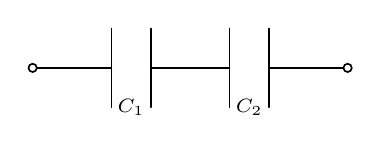
\begin{tikzpicture}[%
        line width=0.6pt,
        line cap=round
    ]
        %   Use this scope to mark circles for the start and end of the circuit.
        \begin{scope}[
            every node/.style={
                circle,
                fill=white,
                draw=black,
                inner sep=0pt,
                minimum size=3pt
            }
        ]
            \node (a) at (0,0) {};
            \node (b) at (4,0) {};
        \end{scope}

        %   Draw the circuit.
        \draw (a) to (1.0, 0.0);
        \draw (1.0, -0.5) to (1.0, 0.5);
        \draw (1.5, -0.5) to (1.5, 0.5);
        \draw (1.5, 0.0) to (2.5, 0.0);
        \draw (2.5, -0.5) to (2.5, 0.5);
        \draw (3.0, -0.5) to (3.0, 0.5);
        \draw (3.0, 0.0) to (b);

        %   Label the plates.
        \node at (1.25,-0.5){\scriptsize{$C_{1}$}};
        \node at (2.75,-0.5){\scriptsize{$C_{2}$}};
    \end{tikzpicture}
\end{document}
